\documentclass[11pt,a4paper]{article}
\usepackage[margin=24mm,headheight=15pt]{geometry}
\usepackage[T1]{fontenc}
\usepackage[utf8]{inputenc}
\usepackage{lmodern,amsmath,amssymb,mathtools}
\usepackage{graphicx,booktabs,longtable,array,calc}
\usepackage{microtype,enumitem,needspace,etoolbox,titlesec}
\usepackage{xcolor,xurl,hyperref,fancyhdr}
\definecolor{noteblue}{HTML}{1458A6}
\hypersetup{colorlinks=true,urlcolor=noteblue,linkcolor=noteblue,pdftitle={Calculus - Week 2},pdfauthor={Jiayu Chen}}
\setlength{\parindent}{0pt}
\setlength{\parskip}{7pt plus 2pt minus 1pt}
\linespread{1.12}
\setlength{\emergencystretch}{3em}
\setlength{\abovedisplayskip}{12pt plus 3pt minus 2pt}
\setlength{\belowdisplayskip}{12pt plus 3pt minus 2pt}
\setlist{itemsep=6pt,topsep=8pt,parsep=3pt,leftmargin=1.8em}
\providecommand{\tightlist}{}
\newcommand{\passthrough}[1]{#1}
\newcommand{\pandocbounded}[1]{#1}
\setcounter{secnumdepth}{0}
\setcounter{tocdepth}{1}
\titleformat{\section}{\Large\bfseries}{\thesection}{0pt}{}
\titleformat{\subsection}{\large\bfseries}{\thesubsection}{0pt}{}
\titleformat{\subsubsection}{\normalsize\bfseries}{\thesubsubsection}{0pt}{}
\titlespacing*{\section}{0pt}{22pt}{12pt}
\titlespacing*{\subsection}{0pt}{18pt}{9pt}
\titlespacing*{\subsubsection}{0pt}{15pt}{7pt}
\pretocmd{\section}{\Needspace{8\baselineskip}}{}{}
\pretocmd{\subsection}{\Needspace{6\baselineskip}}{}{}
\pretocmd{\subsubsection}{\Needspace{5\baselineskip}}{}{}
\pagestyle{fancy}\fancyhf{}
\fancyhead[L]{\small Calculus}
\fancyhead[R]{\small Calculus - Week 2}
\fancyfoot[C]{\small\thepage}
\renewcommand{\headrulewidth}{0.3pt}
\begin{document}
{\LARGE\bfseries Calculus - Week 2\par}
\vspace{5pt}
{\large Continuity, infinity and sequences · Tutorial 1 and Lectures
5--7\par}
\vspace{8pt}
{\small Jiayu Chen\par}
\vspace{10pt}
\tableofcontents
\vspace{16pt}
Week 1 supplied the definition of a limit. Here we use it in three
settings: continuity on an interval, behavior at infinity, and
sequences. The same estimates keep reappearing; what changes is whether
we choose a radius around a point or a threshold beyond which the
estimate holds.

\section{Tutorial 1: proof and
quantifiers}\label{tutorial-1-proof-and-quantifiers}

\subsection{1 Proof, logic, and limit
language}\label{proof-logic-and-limit-language}

\subsubsection{1.1 Basic terminology}\label{basic-terminology}

\begin{itemize}
\item
  An axiom is accepted as part of the framework in which we work.
\item
  A theorem is established by proof; propositions and lemmas have the
  same logical status, with names that describe their role.
\item
  A proof is a finite, logically valid argument using definitions,
  axioms and results already proved.
\item
  In \(P\Rightarrow Q\), \(P\) is the hypothesis and \(Q\) is the
  conclusion. The converse \(Q\Rightarrow P\) requires its own proof.
\end{itemize}

\subsubsection{\texorpdfstring{1.2 The \(\varepsilon\)-\(\delta\)
definition}{1.2 The \textbackslash varepsilon-\textbackslash delta definition}}\label{the-varepsilon-delta-definition}

Here \(\delta\) controls how close the input \(x\) is to \(x_0\), while
\(\varepsilon\) prescribes how close \(f(x)\) must be to \(\ell\).

A standard proof has the following shape:

\begin{enumerate}
\def\labelenumi{\arabic{enumi}.}
\item
  Let \(\varepsilon>0\) be arbitrary.
\item
  Choose an explicit \(\delta>0\), usually after estimating
  \(|f(x)-\ell|\) in terms of \(|x-x_0|\).
\item
  Assume \(0<|x-x_0|<\delta\) and verify \(|f(x)-\ell|<\varepsilon\).
\end{enumerate}

Working backward helps find a suitable radius, but the written proof
should then run forward from that choice. A list of inequalities ending
in a proposed \(\delta\) is not yet the verification.

\subsubsection{1.3 Direct proof, contradiction, and
contraposition}\label{direct-proof-contradiction-and-contraposition}

\paragraph{Direct proof}\label{direct-proof}

To prove a statement of the form

\[
P\Rightarrow Q,
\]

assume that \(P\) is true and use definitions, axioms, and previously
proved results until \(Q\) follows. This is the default method for most
\(\varepsilon\)-\(\delta\) arguments.

\paragraph{Proof by contradiction}\label{proof-by-contradiction}

To prove a statement \(S\):

\begin{enumerate}
\def\labelenumi{\arabic{enumi}.}
\item
  Assume its negation, \(\neg S\).
\item
  Derive a contradiction, such as \(R\land\neg R\), an impossible
  inequality, or a conflict with a known theorem.
\item
  Conclude that \(\neg S\) is false, so \(S\) is true.
\end{enumerate}

For a uniqueness statement, assume that two distinct objects both
satisfy the defining property. For a nonexistence statement, assume that
the object exists and use its required properties to obtain a
contradiction.

\paragraph{\texorpdfstring{Example: irrationality of
\(\sqrt2\)}{Example: irrationality of \textbackslash sqrt2}}\label{example-irrationality-of-sqrt2}

Suppose, for contradiction, that

\[
\sqrt2=\frac{p}{q},
\]

where \(p,q\) are positive integers with no common factor. Squaring
gives

\[
p^2=2q^2.
\]

Thus \(p^2\) is even, so \(p\) is even. Write \(p=2r\). Substitution
gives

\[
4r^2=2q^2
\quad\Longrightarrow\quad
q^2=2r^2.
\]

Therefore \(q\) is also even. Hence \(p\) and \(q\) have the common
factor \(2\), contradicting the assumption that \(p/q\) is in lowest
terms. Consequently,

\[
\sqrt2\notin\mathbb{Q}.
\]

\paragraph{Proof by contraposition}\label{proof-by-contraposition}

To prove

\[
P\Rightarrow Q,
\]

it is enough to prove the logically equivalent statement

\[
\neg Q\Rightarrow\neg P.
\]

This method is especially useful when the negation of the conclusion
gives more concrete information than the conclusion itself.

\subsubsection{1.4 Mathematical induction}\label{mathematical-induction}

Let \(P(n)\) be a statement for \(n\in\mathbb{Z}_{>0}\). The principle
of mathematical induction says that if:

\begin{enumerate}
\def\labelenumi{\arabic{enumi}.}
\item
  \textbf{Base case:} \(P(1)\) is true;
\item
  \textbf{Inductive step:} for every positive integer \(n\), assuming
  \(P(n)\) is true implies that \(P(n+1)\) is true;
\end{enumerate}

then \(P(n)\) is true for every positive integer \(n\).

In the inductive step, clearly state the \textbf{induction hypothesis}
\(P(n)\) before proving \(P(n+1)\). Do not assume the statement that is
being proved.

\paragraph{\texorpdfstring{Example: sum of the first \(n\) positive
integers}{Example: sum of the first n positive integers}}\label{example-sum-of-the-first-n-positive-integers}

We prove that

\[
1+2+\cdots+n=\frac{n(n+1)}{2}
\qquad(n\geq1).
\]

For \(n=1\), both sides equal \(1\). Now assume the formula holds for
\(n=k\):

\[
1+2+\cdots+k=\frac{k(k+1)}{2}.
\]

Then

\[
\begin{aligned}
1+2+\cdots+k+(k+1)
&=\frac{k(k+1)}{2}+(k+1)\\
&=\frac{(k+1)(k+2)}{2}.
\end{aligned}
\]

Thus, the statement for \(k\) implies the statement for \(k+1\), so the
formula holds for every \(n\geq1\).

\paragraph{Strong induction}\label{strong-induction}

The principle of strong induction replaces the induction hypothesis
\(P(n)\) by

\[
P(1),P(2),\ldots,P(n)\quad\Longrightarrow\quad P(n+1).
\]

It is useful when the case \(n+1\) depends on several earlier cases
rather than only on the immediately preceding case.

Ordinary induction, strong induction, and the well-ordering principle
are equivalent principles. The well-ordering principle states that every
nonempty subset of \(\mathbb{Z}_{>0}\) has a least element.

\section{Lecture 5: continuous functions and intermediate
values}\label{lecture-5-continuous-functions-and-intermediate-values}

\subsection{Composition and change of
variable}\label{composition-and-change-of-variable}

\textbf{Continuity of a composition.} If \(g(x)\to b\) as \(x\to c\),
and \(f\) is continuous at \(b\), with \(f(g(x))\) defined near \(c\),
then

\[
\lim_{x\to c}f(g(x))=f(b).
\]

Given \(\varepsilon>0\), continuity of \(f\) gives an input tolerance
\(\eta>0\). The limit of \(g\) then supplies \(\delta\) such that
\(0<|x-c|<\delta\) implies \(|g(x)-b|<\eta\), which in turn implies
\(|f(g(x))-f(b)|<\varepsilon\). If \(g(x)=b\), continuity still covers
that value.

If we assume only \(f(t)\to A\) as \(t\to b\), rather than continuity at
\(b\), we need \(g(x)\ne b\) on a punctured neighborhood. For example,
take \(f(t)=1\) for \(t\ne0\), \(f(0)=0\), and \(g(x)=0\). Then
\(f(t)\to1\) at zero, but \(f(g(x))=0\).

A two-way substitution requires more than \(u(t)\to c\). If \(u\) is a
continuous bijection between neighborhoods of \(t_0\) and \(c\), with
\(u(t_0)=c\) and continuous inverse, the two compositions give

\[
\lim_{x\to c}f(x)=A\quad\Longleftrightarrow\quad
\lim_{t\to t_0}f(u(t))=A.
\]

Squaring near zero is not such a change of variable on a two-sided
interval: it loses the negative side.

\subsection{The Intermediate Value
Theorem}\label{the-intermediate-value-theorem}

If \(f\) is continuous on \([a,b]\), every value between \(f(a)\) and
\(f(b)\) is attained at some point in \([a,b]\). In particular, opposite
signs at the endpoints imply a zero in \((a,b)\).

The theorem gives existence, not uniqueness. A sign change is
sufficient, not necessary: \(x^2\) has a zero without changing sign.
Continuity is essential; a step function can jump across zero without
taking the value zero.

\subsection{Exercise 1.1.26}\label{exercise-1.1.26}

Any polynomial of odd degree with real coefficients has at least one
real root.

\subsubsection{Proof}\label{proof}

Let

\[
P(x)=\sum_{k=0}^{n}a_kx^k
\]

be a polynomial of degree \(n\) with real coefficients, where \(n\) is
an odd integer and \(a_n\neq0\). Without loss of generality, assume that
\(a_n>0\). If \(a_n<0\), we can apply the same argument to \(-P\).

Let

\[
C=\max_{0\leq k\leq n-1}|a_k|.
\]

For \(|x|\geq1\), we have

\[
\begin{aligned}
\left|P(x)-a_nx^n\right|
&=\left|\sum_{k=0}^{n-1}a_kx^k\right|\\
&\leq C\sum_{k=0}^{n-1}|x|^k\\
&\leq Cn|x|^{n-1}
=\frac{Cn}{|a_n||x|}|a_nx^n|.
\end{aligned}
\]

Choose

\[
R>\max\left\{1,\frac{2Cn}{|a_n|}\right\}.
\]

Then, whenever \(|x|\geq R\),

\[
\left|P(x)-a_nx^n\right|<\frac12|a_nx^n|.
\]

Since \(n\) is odd, \(R^n>0\) and \((-R)^n<0\). For \(x=R\), we obtain

\[
\begin{aligned}
P(R)
&\geq a_nR^n-\left|P(R)-a_nR^n\right|\\
&>a_nR^n-\frac12|a_nR^n|
=\frac12a_nR^n>0.
\end{aligned}
\]

For \(x=-R\), we obtain

\[
\begin{aligned}
P(-R)
&\leq a_n(-R)^n+\left|P(-R)-a_n(-R)^n\right|\\
&<a_n(-R)^n+\frac12|a_n(-R)^n|
=\frac12a_n(-R)^n<0.
\end{aligned}
\]

Thus,

\[
P(-R)<0<P(R).
\]

Because \(P\) is continuous on \([-R,R]\), the Intermediate Value
Theorem gives some \(c\in[-R,R]\) such that

\[
P(c)=0.
\]

Therefore, \(P\) has at least one real root. \(\square\)

\subsubsection{Proof of the Intermediate Value
Theorem}\label{proof-of-the-intermediate-value-theorem}

Let \(f\) be continuous on \([a,b]\), and suppose first that

\[
f(a)<y_0<f(b).
\]

Define

\[
S=\{x\in[a,b]:f(x)\leq y_0\}.
\]

The set \(S\) is nonempty because \(a\in S\), and it is bounded above by
\(b\). By the completeness of \(\mathbb{R}\), the supremum

\[
c=\sup S
\]

exists. Continuity at \(a\) gives a short interval \([a,a+\eta]\) on
which \(f<y_0\); continuity at \(b\) gives a short interval
\([b-\eta,b]\) on which \(f>y_0\), after reducing \(\eta>0\) if needed.
Thus \(a+\eta\le c\le b-\eta\), so \(a<c<b\). This is the endpoint step
needed before using a two-sided neighborhood of \(c\).

We claim that \(f(c)=y_0\). Suppose first that \(f(c)<y_0\). By
continuity of \(f\) at \(c\), there exists \(\delta>0\) such that

\[
|x-c|<\delta\quad\Longrightarrow\quad f(x)<y_0.
\]

Choosing \(x>c\) sufficiently close to \(c\) gives \(x\in S\),
contradicting the fact that \(c\) is an upper bound of \(S\).

On the other hand, suppose that \(f(c)>y_0\). By continuity of \(f\) at
\(c\), there exists \(\delta>0\) such that

\[
|x-c|<\delta\quad\Longrightarrow\quad f(x)>y_0.
\]

Since \(c=\sup S\), there is some \(x\in S\) with \(c-\delta<x\leq c\).
This contradicts \(f(x)>y_0\).

Therefore neither \(f(c)<y_0\) nor \(f(c)>y_0\) is possible, and hence

\[
f(c)=y_0.
\]

If \(y_0=f(a)\) or \(y_0=f(b)\), the conclusion is immediate by taking
\(c=a\) or \(c=b\). If \(f(b)<f(a)\), apply the same argument to \(-f\).
Therefore, for every value \(y_0\) between \(f(a)\) and \(f(b)\), there
exists \(c\in[a,b]\) such that

\[
f(c)=y_0.
\]

\section{Lecture 6: infinity and
asymptotes}\label{lecture-6-infinity-and-asymptotes}

\subsection{Limits Involving Infinity}\label{limits-involving-infinity}

\subsubsection{\texorpdfstring{Finite limits as
\(x\to+\infty\)}{Finite limits as x\textbackslash to+\textbackslash infty}}\label{finite-limits-as-xtoinfty}

We say that

\[
\lim_{x\to+\infty}f(x)=L
\]

if, for every \(\varepsilon>0\), there exists \(M>0\) such that

\[
x>M\quad\Longrightarrow\quad |f(x)-L|<\varepsilon.
\]

In words, \(f(x)\) becomes arbitrarily close to \(L\) when \(x\) is
sufficiently large.

Similarly,

\[
\lim_{x\to-\infty}f(x)=L
\]

if, for every \(\varepsilon>0\), there exists \(M<0\) such that

\[
x<M\quad\Longrightarrow\quad |f(x)-L|<\varepsilon.
\]

\subsubsection{Examples}\label{examples}

For the reciprocal function,

\[
\lim_{x\to+\infty}\frac{1}{x}=0,
\qquad
\lim_{x\to-\infty}\frac{1}{x}=0.
\]

Indeed, if \(|x|>1/\varepsilon\), then

\[
\left|\frac{1}{x}-0\right|=\frac{1}{|x|}<\varepsilon.
\]

For a rational function whose numerator has lower degree than its
denominator,

\[
\lim_{x\to\pm\infty}\frac{P(x)}{Q(x)}=0,
\qquad \deg P<\deg Q.
\]

\subsubsection{\texorpdfstring{Infinite limits as
\(x\to c\)}{Infinite limits as x\textbackslash to c}}\label{infinite-limits-as-xto-c}

We write

\[
\lim_{x\to c}f(x)=+\infty
\]

if, for every \(A>0\), there exists \(\delta>0\) such that

\[
0<|x-c|<\delta
\quad\Longrightarrow\quad
f(x)>A.
\]

Similarly,

\[
\lim_{x\to c}f(x)=-\infty
\]

if, for every \(B>0\), there exists \(\delta>0\) such that

\[
0<|x-c|<\delta
\quad\Longrightarrow\quad
f(x)<-B.
\]

For example,

\[
\lim_{x\to0}\frac{1}{x^2}=+\infty,
\]

because \(1/x^2\) can be made larger than any prescribed positive number
by choosing \(x\) sufficiently close to \(0\), with \(x\neq0\).

\subsubsection{\texorpdfstring{Infinite limits as
\(x\to\pm\infty\)}{Infinite limits as x\textbackslash to\textbackslash pm\textbackslash infty}}\label{infinite-limits-as-xtopminfty}

The notation

\[
\lim_{x\to+\infty}f(x)=+\infty
\]

means that for every \(A>0\), there exists \(M>0\) such that

\[
x>M\quad\Longrightarrow\quad f(x)>A.
\]

The other cases are defined analogously. For instance, if \(n\) is odd
and \(a_n>0\), then

\[
\lim_{x\to+\infty}a_nx^n=+\infty,
\qquad
\lim_{x\to-\infty}a_nx^n=-\infty.
\]

\subsection{Exercise 1.1.30}\label{exercise-1.1.30}

\subsubsection{(a)}\label{a}

Prove, using the \(N\)-\(\delta\) language, that

\[
\lim_{x\to0^+}\frac{1}{\sqrt[3]{x}}=+\infty.
\]

\subsubsection{(b)}\label{b}

Find the limit

\[
\lim_{x\to+\infty}\left(\sqrt{x+1}-\sqrt{x-1}\right),
\]

and prove your result using the \(\varepsilon\)-\(N\) language.

\subsubsection{Solution}\label{solution}

\paragraph{(a)}\label{a-1}

Let \(N>0\) be arbitrary. Choose

\[
\delta=\frac{1}{N^3}.
\]

If \(0<x<\delta\), then

\[
\sqrt[3]{x}<\sqrt[3]{\delta}=\frac{1}{N}.
\]

Therefore,

\[
\frac{1}{\sqrt[3]{x}}>\frac{1}{\sqrt[3]{\delta}}=N.
\]

Hence, for every \(N>0\), there exists \(\delta>0\) such that

\[
0<x<\delta
\quad\Longrightarrow\quad
\frac{1}{\sqrt[3]{x}}>N.
\]

Thus,

\[
\boxed{\displaystyle\lim_{x\to0^+}\frac{1}{\sqrt[3]{x}}=+\infty}.
\]

\paragraph{(b)}\label{b-1}

Let

\[
f(x)=\sqrt{x+1}-\sqrt{x-1}.
\]

For \(x\geq1\), rationalizing gives

\[
f(x)
=\frac{(x+1)-(x-1)}{\sqrt{x+1}+\sqrt{x-1}}
=\frac{2}{\sqrt{x+1}+\sqrt{x-1}}.
\]

Since \(\sqrt{x+1}+\sqrt{x-1}\to+\infty\) as \(x\to+\infty\), we obtain

\[
\lim_{x\to+\infty}f(x)=0.
\]

To prove this using the \(\varepsilon\)-\(N\) language, let
\(\varepsilon>0\) be given. Choose

\[
N=1+\frac{1}{\varepsilon^2}.
\]

If \(x>N\), then \(x>1\) and

\[
0<f(x)
=\frac{2}{\sqrt{x+1}+\sqrt{x-1}}
\leq\frac{1}{\sqrt{x-1}}.
\]

Moreover, \(x>N\) implies \(x-1>1/\varepsilon^2\), so

\[
\left|f(x)-0\right|=f(x)
\leq\frac{1}{\sqrt{x-1}}<\varepsilon.
\]

Therefore, for every \(\varepsilon>0\), there exists \(N>0\) such that

\[
x>N\quad\Longrightarrow\quad
\left|\sqrt{x+1}-\sqrt{x-1}\right|<\varepsilon.
\]

Hence,

\[
\boxed{\displaystyle
\lim_{x\to+\infty}\left(\sqrt{x+1}-\sqrt{x-1}\right)=0}.
\]

\subsection{Exercise 1.1.28}\label{exercise-1.1.28}

All the Limit Laws remain true when we replace

\[
\lim_{x\to c}
\]

by

\[
\lim_{x\to+\infty}
\quad\text{or}\quad
\lim_{x\to-\infty}.
\]

For example, if

\[
\lim_{x\to+\infty}f(x)=L,
\qquad
\lim_{x\to+\infty}g(x)=M,
\]

then

\[
\lim_{x\to+\infty}(f(x)+g(x))=L+M,
\]

and, provided \(M\neq0\),

\[
\lim_{x\to+\infty}\frac{f(x)}{g(x)}=\frac{L}{M}.
\]

The same statements hold as \(x\to-\infty\).

\subsection{Asymptotes}\label{asymptotes}

The graph of \(y=f(x)\) on an interval \(I\) is

\[
\{(x,y):x\in I,\ y=f(x)\}.
\]

A line is an asymptote when the graph approaches it along an unbounded
branch. For horizontal and oblique lines we let \(x\) tend to an
infinity. For a vertical line \(x=a\), we require a one-sided infinite
limit of \(f\) at \(a\). Merely having \(x\to a\) is not enough: an
ordinary point of a curve is not a vertical asymptote.

\subsubsection{Horizontal asymptotes}\label{horizontal-asymptotes}

A line \(y=b\) is a horizontal asymptote of \(y=f(x)\) as
\(x\to+\infty\) if

\[
\lim_{x\to+\infty}f(x)=b.
\]

Similarly, \(y=b\) is a horizontal asymptote as \(x\to-\infty\) if

\[
\lim_{x\to-\infty}f(x)=b.
\]

\paragraph{Example 1.1.32}\label{example-1.1.32}

Find the horizontal asymptotes of

\[
f(x)=\frac{\sin x+\cos x}{1+x^2},
\]

and

\[
g(x)=\sqrt{1-\frac{1}{x^2}},\qquad |x|\geq1.
\]

Since \(|\sin x+\cos x|\leq2\),

\[
\left|\frac{\sin x+\cos x}{1+x^2}\right|
\leq\frac{2}{1+x^2}\longrightarrow0.
\]

Thus, \(y=0\) is a horizontal asymptote of \(f\) as \(x\to\pm\infty\).

For \(g\),

\[
\lim_{x\to\pm\infty}g(x)
=\sqrt{1-\lim_{x\to\pm\infty}\frac1{x^2}}
=1.
\]

Thus, \(y=1\) is a horizontal asymptote of \(g\) as \(x\to\pm\infty\).

\subsubsection{Sketches of horizontal
asymptotes}\label{sketches-of-horizontal-asymptotes}

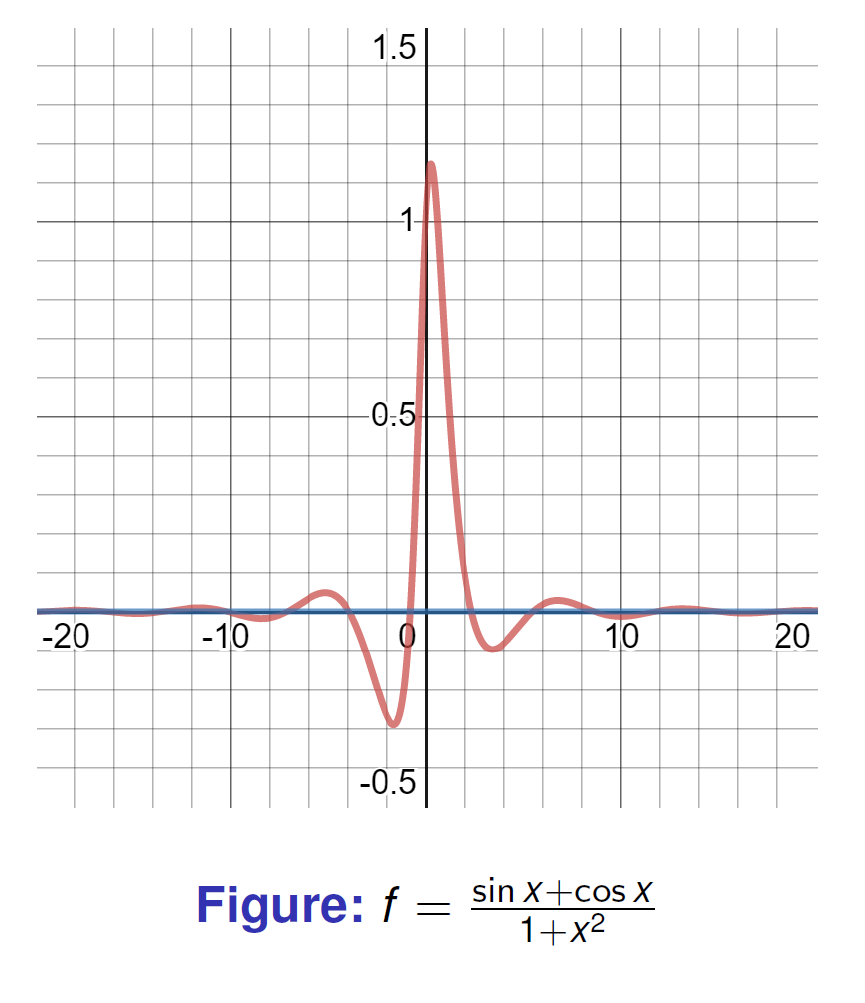
\includegraphics[width=0.65\linewidth,height=\textheight,keepaspectratio]{image-13.png}

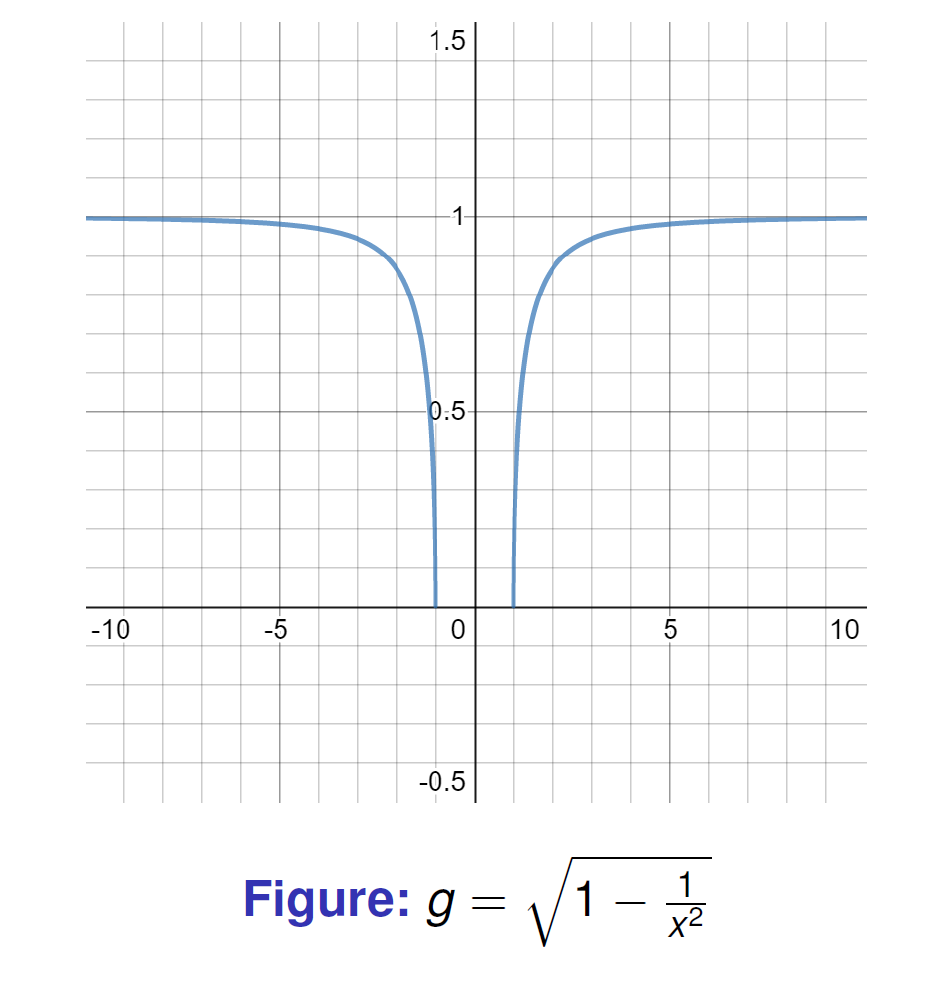
\includegraphics[width=0.65\linewidth,height=\textheight,keepaspectratio]{image-14.png}

\subsubsection{Vertical asymptotes}\label{vertical-asymptotes}

A line \(x=a\) is a vertical asymptote of \(y=f(x)\) as \(x\to a^+\) if

\[
\lim_{x\to a^+}f(x)=+\infty
\quad\text{or}\quad
\lim_{x\to a^+}f(x)=-\infty.
\]

The analogous definition applies as \(x\to a^-\). In the notation
\(\pm\infty\), the sign may be either \(+\) or \(-\).

\paragraph{Example 1.1.33}\label{example-1.1.33}

Consider

\[
h(x)=\sqrt{1-\frac{\sin x}{x^2}},
\]

on its domain

\[
(-\infty,0)\cup[a,+\infty),
\]

where the boundary point \(a>0\) is determined by

\[
a^2=\sin a,
\]

where \(0<a<1\). As \(x\to0^-\), we have \(\sin x\sim x\), and therefore

\[
1-\frac{\sin x}{x^2}
\sim 1-\frac1x\longrightarrow+\infty.
\]

Consequently,

\[
\lim_{x\to0^-}h(x)=+\infty,
\]

so \(x=0\) is a vertical asymptote. Near \(x=a\) from the right, the
expression under the square root approaches \(0\), so \(x=a\) is not a
vertical asymptote.

This example emphasizes that a domain endpoint is not automatically a
vertical asymptote: the function itself must tend to \(\pm\infty\).

\subsubsection{Sketches of vertical
asymptotes}\label{sketches-of-vertical-asymptotes}

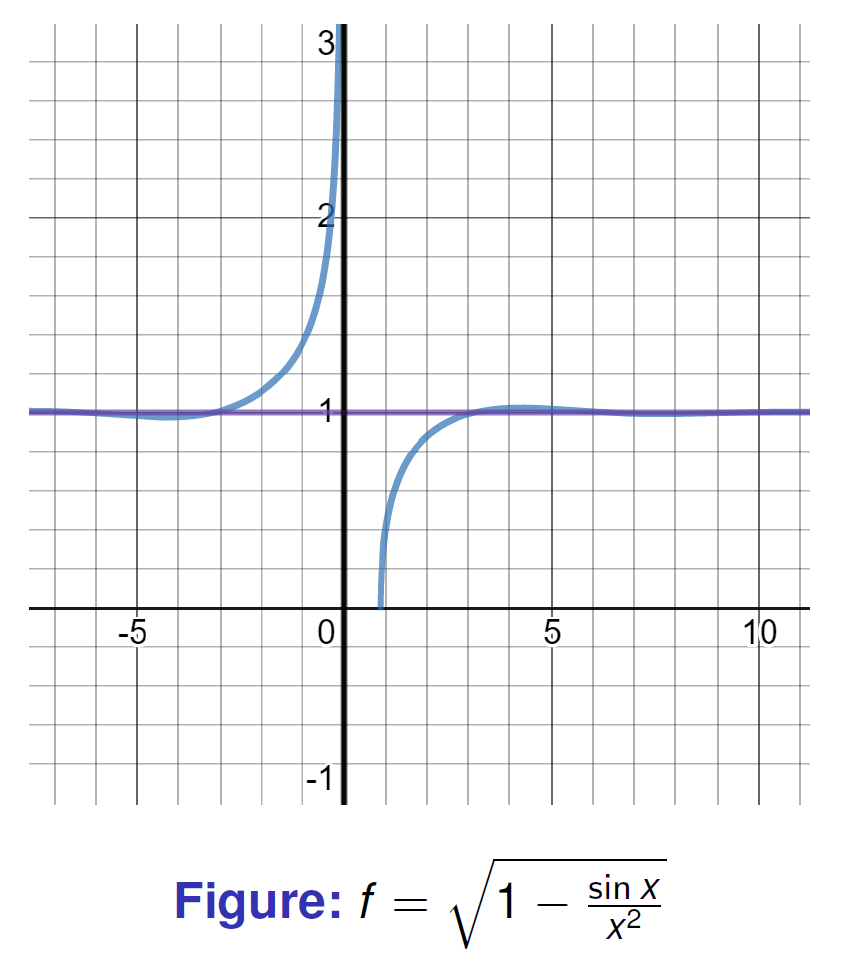
\includegraphics[width=0.65\linewidth,height=\textheight,keepaspectratio]{image-15.png}

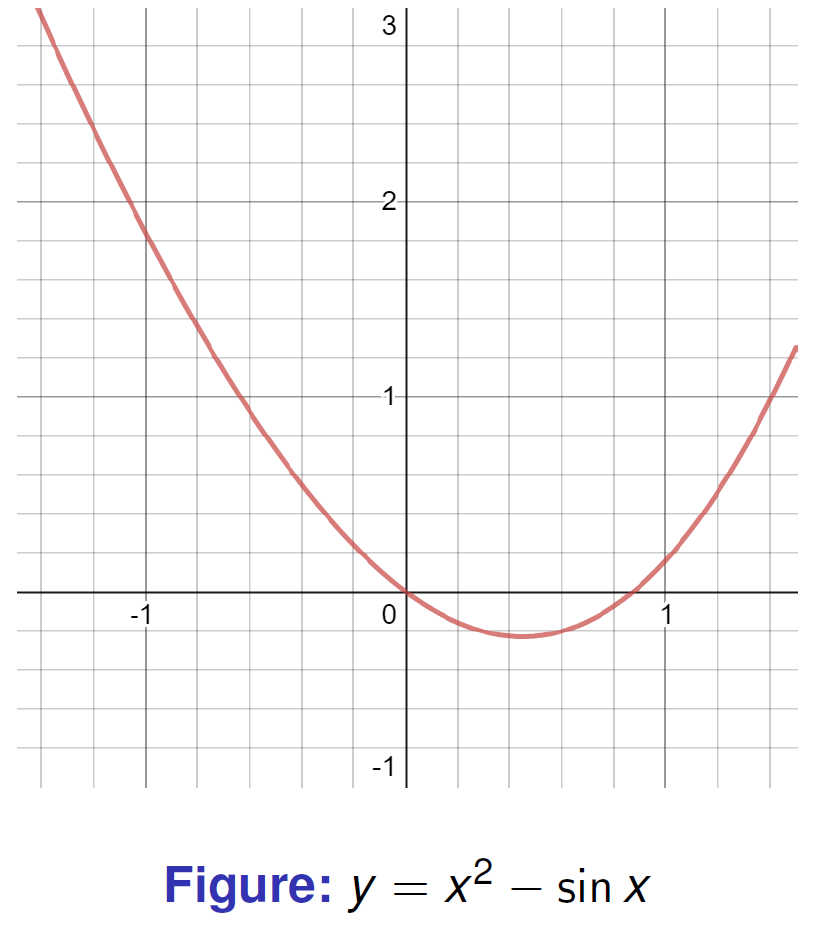
\includegraphics[width=0.65\linewidth,height=\textheight,keepaspectratio]{image-16.png}

\subsubsection{Oblique asymptotes}\label{oblique-asymptotes}

A line

\[
y=ax+b,\qquad a\neq0,
\]

is an oblique asymptote of \(y=f(x)\) as \(x\to+\infty\) if

\[
\lim_{x\to+\infty}[f(x)-ax-b]=0.
\]

The definition as \(x\to-\infty\) is analogous.

When the limits exist, the coefficients can be found from

\[
a=\lim_{x\to\pm\infty}\frac{f(x)}{x},
\qquad
b=\lim_{x\to\pm\infty}[f(x)-ax].
\]

\paragraph{Example 1.1.34}\label{example-1.1.34}

Find the oblique asymptote of

\[
f(x)=\frac{x^2-3}{2x-4}.
\]

Polynomial division gives

\[
\begin{aligned}
f(x)
&=\frac{x^2-4+1}{2(x-2)}\\
&=\frac12(x+2)+\frac{1}{2(x-2)}.
\end{aligned}
\]

Therefore,

\[
f(x)-\left(\frac{x}{2}+1\right)
=\frac{1}{2(x-2)}\longrightarrow0
\qquad(x\to\pm\infty).
\]

The oblique asymptote is

\[
y=\frac{x}{2}+1.
\]

Also, \(x=2\) is a vertical asymptote.

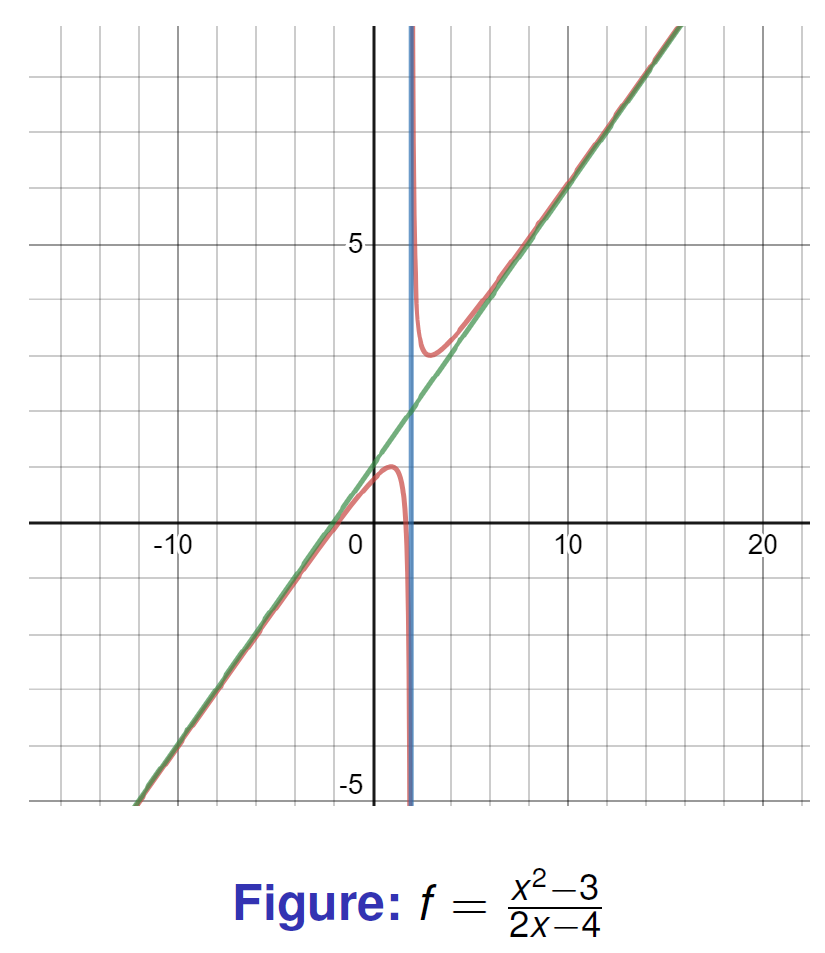
\includegraphics[width=0.65\linewidth,height=\textheight,keepaspectratio]{image-17.png}

\paragraph{Example 1.1.35}\label{example-1.1.35}

Let

\[
f(x)=\frac{x^3}{(x+2)(x-1)}.
\]

The vertical asymptotes are

\[
x=-2,\qquad x=1.
\]

For the oblique asymptote,

\[
\frac{f(x)}{x}
=\frac{x^2}{(x+2)(x-1)}\longrightarrow1,
\]

and

\[
f(x)-x
=\frac{-x^2+2x}{(x+2)(x-1)}\longrightarrow-1.
\]

Hence the oblique asymptote is

\[
y=x-1
\]

as \(x\to\pm\infty\).

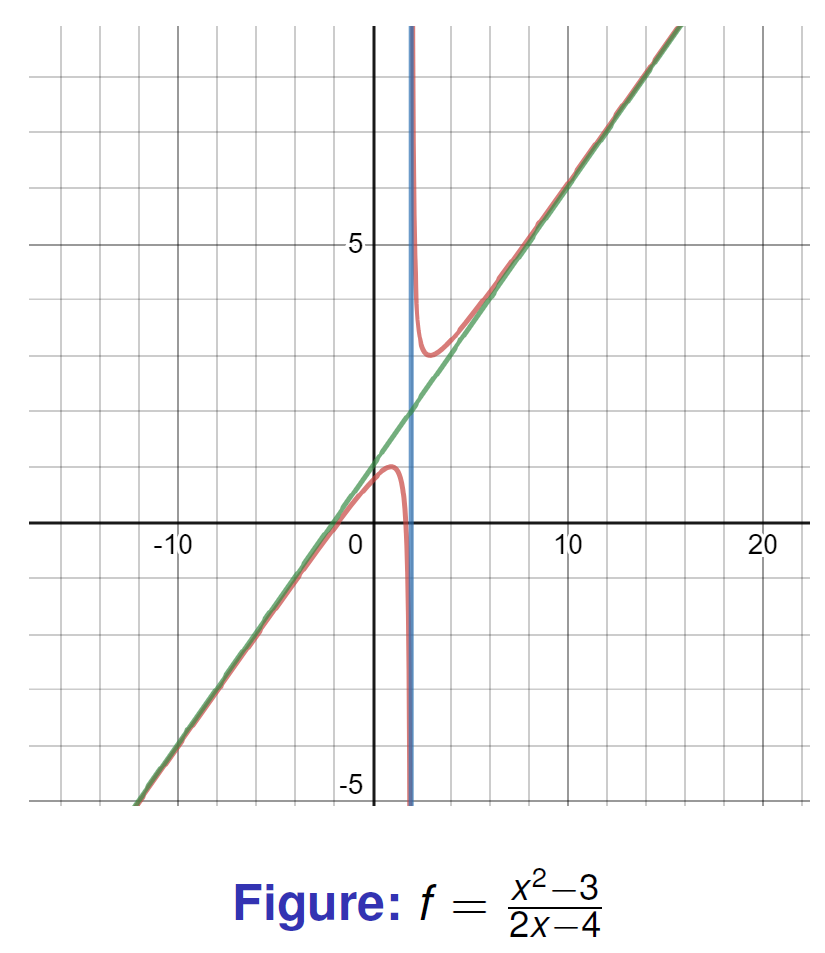
\includegraphics[width=0.65\linewidth,height=\textheight,keepaspectratio]{image-18.png}

\subsection{Exercise 1.1.36}\label{exercise-1.1.36}

Let

\[
f(x)=\frac1x\sin\frac1x.
\]

Does the graph of \(f\) have a vertical asymptote at \(x=0\)? Explain
your answer using the definition of a vertical asymptote.

Since

\[
\left|\frac1x\sin\frac1x\right|\leq\frac1{|x|},
\]

this estimate alone does not determine an infinite limit. To see the
oscillation explicitly, define

\[
x_n=\frac{1}{\frac{\pi}{2}+2\pi n},
\qquad
y_n=\frac{1}{\frac{3\pi}{2}+2\pi n}.
\]

Then \(x_n,y_n\to0^+\) and

\[
f(x_n)=\frac{\pi}{2}+2\pi n\longrightarrow+\infty,
\]

while

\[
f(y_n)=-\left(\frac{3\pi}{2}+2\pi n\right)\longrightarrow-\infty.
\]

Thus, as \(x\to0^+\), the function tends neither to \(+\infty\) nor to
\(-\infty\). Applying the same argument to \(-x_n\) and \(-y_n\) gives
the same conclusion as \(x\to0^-\). Therefore, \(x=0\) is not a vertical
asymptote in the usual one-sided sense.

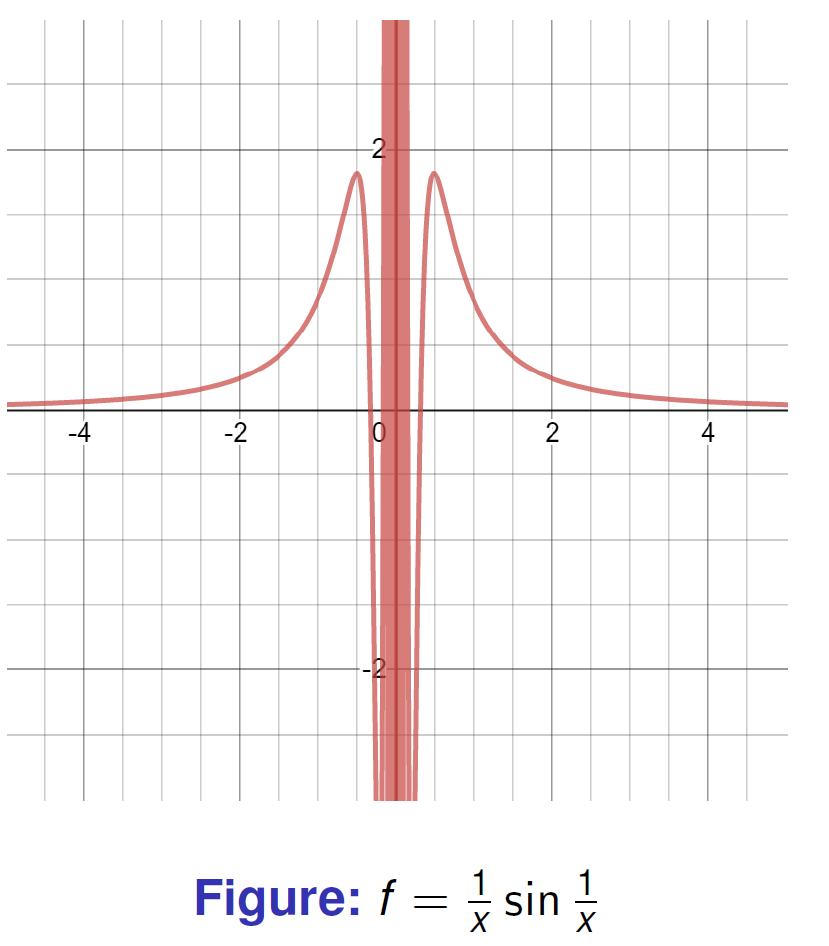
\includegraphics[width=0.65\linewidth,height=\textheight,keepaspectratio]{image-19.png}

\subsection{More Exercises}\label{more-exercises}

Find the limits and use the \(\varepsilon\)-\(N\) language to prove your
results.

\subsubsection{(a)}\label{a-2}

\[
\lim_{x\to+\infty}\sqrt{x}\left(\sqrt{x+1}-\sqrt{x-1}\right).
\]

\subsubsection{(b)}\label{b-2}

\[
\lim_{x\to+\infty}
\frac{\sqrt{x+\sqrt{x+\sqrt{x}}}}{\sqrt{x+1}}.
\]

\textbf{Solution to (a).} Rationalizing and dividing the denominator by
\(\sqrt{x}\) gives

\[
A(x)=\frac{2}{\sqrt{1+1/x}+\sqrt{1-1/x}}\longrightarrow1.
\]

For \(x\ge2\), write \(S=\sqrt{1+1/x}+\sqrt{1-1/x}\ge1\). Rationalizing
each difference from \(1\) shows \(|S-2|\le2/x\), so \(|A(x)-1|\le2/x\).
The choice \(N=\max\{2,2/\varepsilon\}\) verifies the limit directly.

\textbf{Solution to (b).} The denominator is outside the outer radical,
as in Lecture 6, p.32. Put

\[
B(x)=\sqrt{\frac{x+\sqrt{x+\sqrt{x}}}{x+1}},\qquad x\ge1.
\]

Then \(B(x)\to1\). To obtain a threshold rather than only a formal
calculation, use

\[
|B(x)-1|
=\frac{\sqrt{x+\sqrt{x}}-1}{(x+1)(B(x)+1)}
\le\frac{\sqrt{2x}}{x+1}\le\frac{\sqrt2}{\sqrt{x}}.
\]

Thus \(N=\max\{1,2/\varepsilon^2\}\) works. Moving the denominator
inside the radical would change the problem.

\section{Lecture 7: sequences and
completeness}\label{lecture-7-sequences-and-completeness}

\subsection{1.7 Sequences and limits}\label{sequences-and-limits}

\subsubsection{Definition 1.1.12 (Limit of a
sequence)}\label{definition-1.1.12-limit-of-a-sequence}

A sequence \(\{a_n\}\) converges to \(L\) if for every \(\varepsilon>0\)
there exists an integer \(N\) such that

\[
n>N \quad\Longrightarrow\quad |a_n-L|<\varepsilon.
\]

If no such number \(L\) exists, we say that the sequence diverges.

We write

\[
\lim_{n\to\infty}a_n=L,
\qquad\text{or}\qquad a_n\to L.
\]

\subsubsection{Exercise 1.1.39}\label{exercise-1.1.39}

Show that if a sequence converges, then the limit is unique.

\paragraph{Proof}\label{proof-1}

Suppose that

\[
a_n\to L_1,
\qquad a_n\to L_2.
\]

Let \(\varepsilon>0\) be arbitrary. Then there exist \(N_1,N_2\) such
that

\[
n>N_1 \Rightarrow |a_n-L_1|<\varepsilon/2,
\]

and

\[
n>N_2 \Rightarrow |a_n-L_2|<\varepsilon/2.
\]

For \(n>\max\{N_1,N_2\}\),

\[
|L_1-L_2|
\le |a_n-L_1|+|a_n-L_2|
< \varepsilon.
\]

Since this holds for every \(\varepsilon>0\), we must have \(L_1=L_2\).

Hence the limit is unique.

\subsubsection{Example 1.1.40}\label{example-1.1.40}

Investigate the convergence or divergence of the following sequences.

\paragraph{\texorpdfstring{(a) \((-1)^n\)}{(a) (-1)\^{}n}}\label{a--1n}

This sequence alternates between \(-1\) and \(1\), so it does not
approach any single number. Therefore,

\[
(-1)^n\text{ diverges.}
\]

\paragraph{\texorpdfstring{(b)
\(\displaystyle \frac{\sin n-n^2}{n^3+1}\)}{(b) \textbackslash displaystyle \textbackslash frac\{\textbackslash sin n-n\^{}2\}\{n\^{}3+1\}}}\label{b-displaystyle-fracsin-n-n2n31}

Since

\[
\frac{\sin n-n^2}{n^3+1}
=
\frac{\sin n}{n^3+1}-\frac{n^2}{n^3+1},
\]

and both terms go to \(0\), we have

\[
\lim_{n\to\infty}\frac{\sin n-n^2}{n^3+1}=0.
\]

\paragraph{\texorpdfstring{(c)
\(\displaystyle \frac{(-1)^{[\sqrt n]}}{n}\)}{(c) \textbackslash displaystyle \textbackslash frac\{(-1)\^{}\{{[}\textbackslash sqrt n{]}\}\}\{n\}}}\label{c-displaystyle-frac-1sqrt-nn}

Here \([\sqrt n]\) is the integer part of \(\sqrt n\), and the numerator
is always \(\pm1\). Since dividing by \(n\) makes the magnitude go to
\(0\),

\[
\lim_{n\to\infty}\frac{(-1)^{[\sqrt n]}}{n}=0.
\]

\subsection{Bounded sequences}\label{bounded-sequences}

\subsubsection{Definition}\label{definition}

A sequence \(\{a_n\}\) is called:

\begin{itemize}
\item
  bounded above if there exists a constant \(M\) such that \(a_n\le M\)
  for all \(n\);
\item
  bounded below if there exists a constant \(m\) such that \(a_n\ge m\)
  for all \(n\);
\item
  bounded if there exists a constant \(C>0\) such that \(|a_n|\le C\)
  for all \(n\).
\end{itemize}

Equivalently, \(\{a_n\}\) is bounded iff there exist \(m,M\) with

\[
m\le a_n\le M \qquad \forall n\ge1.
\]

\subsubsection{Theorem}\label{theorem}

Every convergent sequence is bounded.

\paragraph{Proof}\label{proof-2}

If \(a_n\to L\), then for \(\varepsilon=1\) there exists \(N\) such that

\[
n>N \Rightarrow |a_n-L|<1.
\]

Thus for all \(n>N\),

\[
|a_n|\le |L|+1.
\]

Let

\[
C=\max\{|a_1|,\dots,|a_N|,|L|+1\}.
\]

Then \(|a_n|\le C\) for all \(n\), so the sequence is bounded.

\subsection{Divergence to infinity}\label{divergence-to-infinity}

\subsubsection{Definition}\label{definition-1}

We say that \(a_n\to +\infty\) if for every real number \(M\) there
exists an integer \(N\) such that

\[
n\ge N \Rightarrow a_n>M.
\]

We say that \(a_n\to -\infty\) if for every real number \(m>0\) there
exists an integer \(N\) such that

\[
n\ge N\Rightarrow a_n<-m.
\]

\subsubsection{Example 1.1.41}\label{example-1.1.41}

Investigate the behavior of the following sequences as \(n\to\infty\).

\paragraph{\texorpdfstring{(a)
\((-1)^n n\)}{(a) (-1)\^{}n n}}\label{a--1n-n}

This sequence alternates sign and grows in magnitude, so it is unbounded
and does not converge to a finite limit. It also does not tend to
\(+\infty\) or \(-\infty\) in the usual sense because the signs
alternate.

\paragraph{\texorpdfstring{(b) \(a^n/n!\) with
\(a>0\)}{(b) a\^{}n/n! with a\textgreater0}}\label{b-ann-with-a0}

For fixed \(a>0\), set \(b_n=a^n/n!\). For \(n\) large enough,

\[
\frac{b_{n+1}}{b_n}=\frac{a}{n+1}\le\frac12.
\]

Hence \(b_{N+k}\le b_N2^{-k}\to0\). This gives a proof of the statement
that a factorial eventually dominates a fixed exponential:

\[
\frac{a^n}{n!}\to0.
\]

\paragraph{\texorpdfstring{(c) \(n^n/n!\)}{(c) n\^{}n/n!}}\label{c-nnn}

Since

\[
\frac{n^n}{n!}=\prod_{k=1}^n\frac{n}{k},
\]

the factors with \(k\le\lfloor n/2\rfloor\) are at least \(2\), and all
remaining factors are at least \(1\). Consequently

\[
\frac{n^n}{n!}\ge2^{\lfloor n/2\rfloor}\longrightarrow+\infty.
\]

In particular,

\[
\frac{n^n}{n!}\to +\infty.
\]

\subsection{Limit laws for sequences}\label{limit-laws-for-sequences}

If

\[
\lim_{n\to\infty}a_n=A,
\qquad
\lim_{n\to\infty}b_n=B,
\]

then the following hold:

\begin{enumerate}
\def\labelenumi{\arabic{enumi}.}
\item
  \(\displaystyle \lim_{n\to\infty}(a_n+b_n)=A+B\);
\item
  \(\displaystyle \lim_{n\to\infty}(a_n-b_n)=A-B\);
\item
  \(\displaystyle \lim_{n\to\infty}(k a_n)=kA\) for any constant \(k\);
\item
  \(\displaystyle \lim_{n\to\infty}(a_n b_n)=AB\);
\item
  if \(B\neq0\), then
\end{enumerate}

\[
\lim_{n\to\infty}\frac{a_n}{b_n}=\frac{A}{B}.
\]

\subsection{Exercise 1.1.43}\label{exercise-1.1.43}

Let \(\{a_n\}\) and \(\{b_n\}\) be convergent sequences and assume
\(a_n\ge b_n\) for all sufficiently large \(n\). Prove that

\[
\lim_{n\to\infty}a_n\ge \lim_{n\to\infty}b_n.
\]

\subsubsection{Proof}\label{proof-3}

Let

\[
A=\lim_{n\to\infty}a_n,
\qquad B=\lim_{n\to\infty}b_n.
\]

Suppose, for contradiction, that \(A<B\). Set

\[
\varepsilon=\frac{B-A}{2}>0.
\]

Then there exists \(N\) such that for all \(n>N\),

\[
|a_n-A|<\varepsilon,
\qquad |b_n-B|<\varepsilon.
\]

Hence for \(n>N\),

\[
a_n<A+\varepsilon=\frac{A+B}{2},
\]

and

\[
b_n>B-\varepsilon=\frac{A+B}{2}.
\]

So \(a_n<b_n\) for all sufficiently large \(n\), contradicting the
assumption that \(a_n\ge b_n\) eventually. Therefore,

\[
A\ge B.
\]

\subsection{Exercise 1.1.43
(continued)}\label{exercise-1.1.43-continued}

Assume \(a_n\le b_n\le c_n\) for all \(n\ge N_0\) and

\[
\lim_{n\to\infty}a_n = \lim_{n\to\infty}c_n = L.
\]

Then

\[
\lim_{n\to\infty}b_n = L.
\]

\subsubsection{Proof}\label{proof-4}

Let \(\varepsilon>0\) be given. Since \(a_n\to L\) and \(c_n\to L\),
there exist \(N_1,N_2\) such that

\[
n>N_1 \Rightarrow |a_n-L|<\varepsilon,
\]

and

\[
n>N_2 \Rightarrow |c_n-L|<\varepsilon.
\]

Let \(N=\max\{N_0,N_1,N_2\}\). Then for all \(n>N\),

\[
L-\varepsilon<a_n\le b_n\le c_n<L+\varepsilon.
\]

Hence

\[
|b_n-L|<\varepsilon,
\]

for all \(n>N\). Therefore, \(b_n\to L\).

This is the sequence version of the Sandwich Theorem.

\subsection{Exercise 1.1.44}\label{exercise-1.1.44}

Let \(\{a_n\}\) be a sequence with \(a_n\to L\), and let \(f\) be a
function continuous at \(L\) and defined at all \(a_n\). Then

\[
f(a_n)\to f(L).
\]

\subsubsection{Proof}\label{proof-5}

Let \(\varepsilon>0\) be given. Since \(f\) is continuous at \(L\),
there exists \(\delta>0\) such that

\[
|x-L|<\delta \Rightarrow |f(x)-f(L)|<\varepsilon.
\]

Because \(a_n\to L\), there exists \(N\) such that

\[
n>N \Rightarrow |a_n-L|<\delta.
\]

Therefore, for all \(n>N\),

\[
|f(a_n)-f(L)|<\varepsilon.
\]

So \(f(a_n)\to f(L)\).

\subsection{Proposition 1.1.13 (function limits and sequence
limits)}\label{proposition-1.1.13-function-limits-and-sequence-limits}

Let \(I\) be an interval containing \(x_0\) in its interior and let
\(f\) be defined on \(I\setminus\{x_0\}\). Then

\[
\lim_{x\to x_0}f(x)=A
\]

exists if and only if for every sequence
\(\{a_n\}\subset I\setminus\{x_0\}\) with \(a_n\to x_0\), the limit

\[
\lim_{n\to\infty}f(a_n)
\]

exists and equals \(A\).

\subsubsection{Proof}\label{proof-6}

\begin{itemize}
\item
  If \(f(x)\to A\), fix \(\varepsilon>0\) and take its limit radius
  \(\delta\). Since \(a_n\to x_0\) with \(a_n\ne x_0\), eventually
  \(0<|a_n-x_0|<\delta\). Hence \(|f(a_n)-A|<\varepsilon\).
\item
  Conversely, suppose the function limit were not \(A\). Negating the
  definition supplies \(\varepsilon_0>0\) such that every radius
  contains a point violating the error bound. For each \(n\), choose
  \(x_n\) with \(0<|x_n-x_0|<1/n\) and \(|f(x_n)-A|\ge\varepsilon_0\).
  Then \(x_n\to x_0\) but \(f(x_n)\) does not converge to \(A\), a
  contradiction.
\end{itemize}

The version in the lecture says only that \(f(a_n)\) converges for every
admissible sequence. The common value then follows too: if two sequences
gave different limits, interleaving them would produce an admissible
sequence whose image does not converge.

Thus, the limit of a function can be tested using sequences.

\subsection{Exercise 1.1.45}\label{exercise-1.1.45}

Let \(f\) be a function defined on \([M,\infty)\). Prove:

\subsubsection{(a)}\label{a-3}

\[
\lim_{x\to\infty}f(x)=L
\]

if and only if for every sequence \(a_n\to\infty\),

\[
\lim_{n\to\infty}f(a_n)=L.
\]

\subsubsection{(b)}\label{b-3}

\[
\lim_{x\to\infty}f(x)=+\infty
\]

if and only if for every sequence \(a_n\to\infty\),

\[
\lim_{n\to\infty}f(a_n)=+\infty.
\]

\textbf{Proof.} The forward implications follow directly from the
threshold definitions. If the finite limit fails, there are
\(\varepsilon_0>0\) and points \(x_n>\max\{M,n\}\) with
\(|f(x_n)-L|\ge\varepsilon_0\). If the infinite limit fails, there are a
fixed bound \(A>0\) and points \(x_n>\max\{M,n\}\) with \(f(x_n)\le A\).
In either case \(x_n\to\infty\) contradicts the corresponding hypothesis
about all sequences.

\subsection{1.8 Least upper bound and greatest lower
bound}\label{least-upper-bound-and-greatest-lower-bound}

\subsubsection{Definition}\label{definition-2}

Let \(\{a_n\}\) be a sequence bounded above. A number \(L\) is called
the least upper bound, or supremum, of \(\{a_n\}\) if:

\begin{enumerate}
\def\labelenumi{\arabic{enumi}.}
\item
  \(a_n\le L\) for all \(n\);
\item
  if \(M\) is any upper bound, then \(L\le M\).
\end{enumerate}

We write

\[
L=\sup_{n\ge1}a_n.
\]

Similarly, if \(\{a_n\}\) is bounded below, a number \(l\) is called the
greatest lower bound, or infimum, if:

\begin{enumerate}
\def\labelenumi{\arabic{enumi}.}
\item
  \(a_n\ge l\) for all \(n\);
\item
  if \(m\) is any lower bound, then \(l\ge m\).
\end{enumerate}

We write

\[
l=\inf_{n\ge1}a_n.
\]

\subsubsection{Remarks}\label{remarks}

\begin{itemize}
\tightlist
\item
  For the supremum: for every \(\varepsilon>0\), there exists \(n\) such
  that
\end{itemize}

\[
a_n>L-\varepsilon.
\]

\begin{itemize}
\tightlist
\item
  For the infimum: for every \(\varepsilon>0\), there exists \(n\) such
  that
\end{itemize}

\[
a_n<l+\varepsilon.
\]

\subsubsection{Theorem 1.1.15}\label{theorem-1.1.15}

Any sequence bounded above has a supremum, and any sequence bounded
below has an infimum.

This is the completeness property of the real numbers.

\subsection{Example 1.1.47}\label{example-1.1.47}

Find the infimum and supremum of the following sequences.

\subsubsection{\texorpdfstring{(a)
\(\left\{(-1)^n/n\right\}_{n\ge1}\)}{(a) \textbackslash left\textbackslash\{(-1)\^{}n/n\textbackslash right\textbackslash\}\_\{n\textbackslash ge1\}}}\label{a-left-1nnright_nge1}

\[
\inf=-1,\qquad \sup=\frac12.
\]

The first term is \(-1\), so an infimum of \(-1/2\) would already fail
to be a lower bound. The odd-indexed terms increase from \(-1\) toward
zero; the even-indexed terms decrease from \(1/2\) toward zero. Both
extremal values are attained.

\subsubsection{\texorpdfstring{(b)
\(\{(-1)^n n\}_{n\ge1}\)}{(b) \textbackslash\{(-1)\^{}n n\textbackslash\}\_\{n\textbackslash ge1\}}}\label{b--1n-n_nge1}

This sequence is unbounded above and below, so

\[
\sup=+\infty,
\qquad\inf=-\infty.
\]

\subsubsection{\texorpdfstring{(c)
\(\{n^{(-1)^n}\}_{n\ge1}\)}{(c) \textbackslash\{n\^{}\{(-1)\^{}n\}\textbackslash\}\_\{n\textbackslash ge1\}}}\label{c-n-1n_nge1}

This is a power, not the product in (b). Even indices give
\(a_{2k}=2k\), whereas odd indices give \(a_{2k-1}=1/(2k-1)\). Therefore

\[
\sup=+\infty,
\qquad\inf=0.
\]

There is no minimum: every term is positive, but the odd subsequence
tends to zero. The product \(n(-1)^n\) in the original transcription is
the same sequence as (b), whose extended bounds are \(-\infty\) and
\(+\infty\).

\subsubsection{\texorpdfstring{(d) \(a_1=\sqrt2\),
\(a_{n+1}=\sqrt{2+a_n}\)}{(d) a\_1=\textbackslash sqrt2, a\_\{n+1\}=\textbackslash sqrt\{2+a\_n\}}}\label{d-a_1sqrt2-a_n1sqrt2a_n}

Induction gives \(0<a_n<2\): if \(a_n<2\), then
\(a_{n+1}=\sqrt{2+a_n}<2\). Also \(a_2>a_1\), and monotonicity of the
square root propagates \(a_{n+1}>a_n\). An increasing, bounded sequence
converges: if \(L=\sup\{a_n\}\), then for every \(\varepsilon>0\) some
term exceeds \(L-\varepsilon\), and all later terms remain between
\(L-\varepsilon\) and \(L\).

Only after proving convergence do we pass to the limit in the
recurrence. Continuity of the square root gives the positive solution of

\[
x=\sqrt{2+x},
\]

namely

\[
x^2-x-2=0 \Rightarrow x=2.
\]

Thus,

\[
\sup=2,
\qquad\inf=\sqrt2.
\]

\subsection{What a bound does, and does not, tell
us}\label{what-a-bound-does-and-does-not-tell-us}

A supremum concerns all terms, including the first few; a limit ignores
any finite initial segment. For instance, changing \(a_1\) to \(100\)
changes the supremum but not a pre-existing limit. Boundedness alone
does not imply convergence, as \((-1)^n\) shows. Monotonicity is the
extra hypothesis in the theorem used for the radical recurrence.

\subsection{Review problems}\label{review-problems}

\begin{enumerate}
\def\labelenumi{\arabic{enumi}.}
\item
  Explain why the IVT cannot establish uniqueness of a root. Identify
  where completeness enters its proof.
\item
  Find both asymptotes of \((x^2-3)/(2x-4)\), and explain why a function
  can cross a horizontal or oblique asymptote.
\item
  Compare \((-1)^n n\), \(n^{(-1)^n}\) and \((-1)^n/n\): determine
  boundedness, convergence, infimum and supremum separately.
\item
  Prove the radical recurrence stays below \(2\) before attempting to
  solve its limiting equation.
\end{enumerate}

\subsection{Lecture sources}\label{lecture-sources}

Xing-Bin Pan, MAT1011 lecture slides: Lecture 5 (continuity of
compositions and intermediate values), Lecture 6 (infinite limits and
asymptotes; the nested-radical exercise is on p.32), Lecture 7
(sequences, pp.3--33; completeness and Example 1.1.47, pp.34--41).
Tutorial 1 supplies the proof-language section. Differentiation begins
in Week 3.
\end{document}
